\section{Additional Discussion on Factors Affecting MAS Performance}
\label{ap:discuss_control}


\subsection{MAS vs. SAS for Robustness Axis}
\label{ap:mas_sas_robustness}


\begin{center}
\vspace{-0.5\baselineskip}
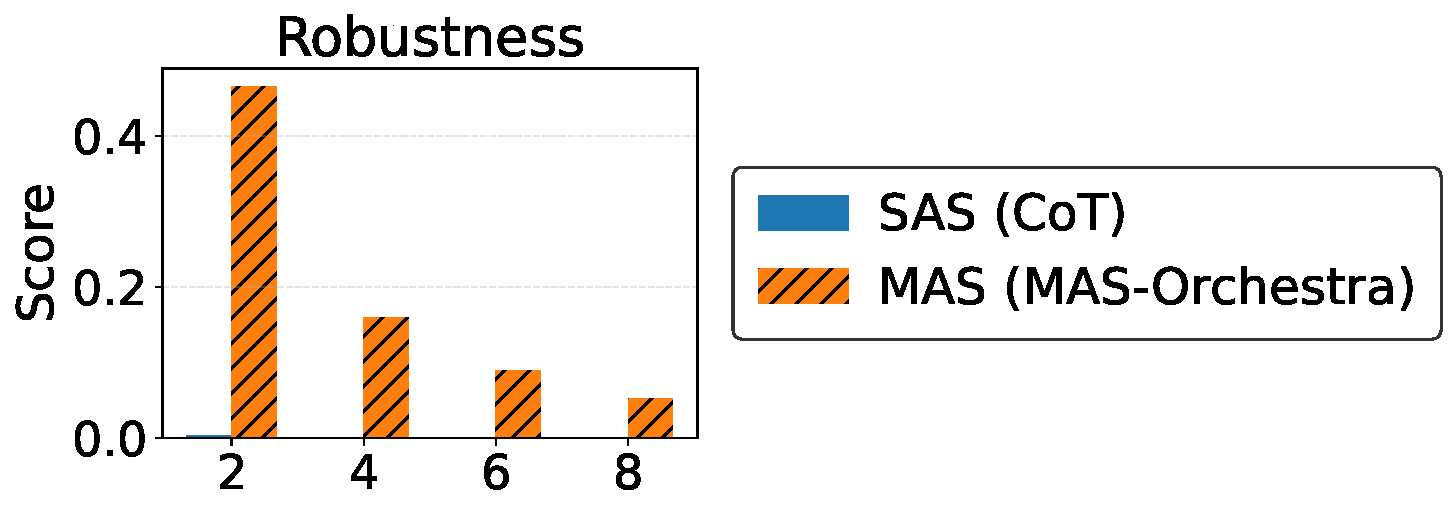
\includegraphics[width=0.5\columnwidth]{figs/oss120b_robustness.pdf}
\vspace{-0.5\baselineskip}
\captionof{figure}{\small \avgat{8} in the  \robustness setting with \ossonetwentylow as the sub-agent. (SAS performance is too low to be visible.)}
% \zixuan{TODO: update the bg color}
\label{fig:robustness}
\end{center}



In \cref{tab:sas_mas_example}, we demonstrate a sample from the \robustness axis (\robustness equals to 2) using \qwen as the orchestrator and \ossonetwenty as the sub-agent (or agent if SAS). See \cref{sec:subtask_structure} for detailed descriptions and observations.

\begin{table*}[h]
\centering
\small
% \addtolength{\tabcolsep}{-0.4em}
\begin{tabularx}{\textwidth}{l X X}
\toprule
 & \textbf{Single-agent System (SAS)} & \textbf{Multi-agent System (MAS)} \\
\midrule
\textbf{Problem}
& \multicolumn{2}{p{0.76\linewidth}}{
From the passage, identify and return (1) the magic number for thundering-autumn and (2) the number of Accordion File that Beach Backpack has, wrapped in \texttt{\textbackslash boxed\{\}} and separated by a double newline.
} \\
\midrule
\textbf{Thinking}
&
We identified the magic number as 7381734 from the note.  
The Insulated Backpack's Accordion File is 21, and the Beach Backpack's Accordion File is twice that, so it is 42.  
The answer consists of two boxed numbers separated by a double newline.
&
The task is decomposed into two sub-problems:  
(1) extract the magic number for thundering-autumn from the passage;  
(2) compute the number of Accordion File that Beach Backpack has using the given relations.  
A sink agent formats the final output.
\\
\midrule
\textbf{MAS Design}
&
N/A
&
\hspace{-50mm}
\raisebox{-0.5\height}{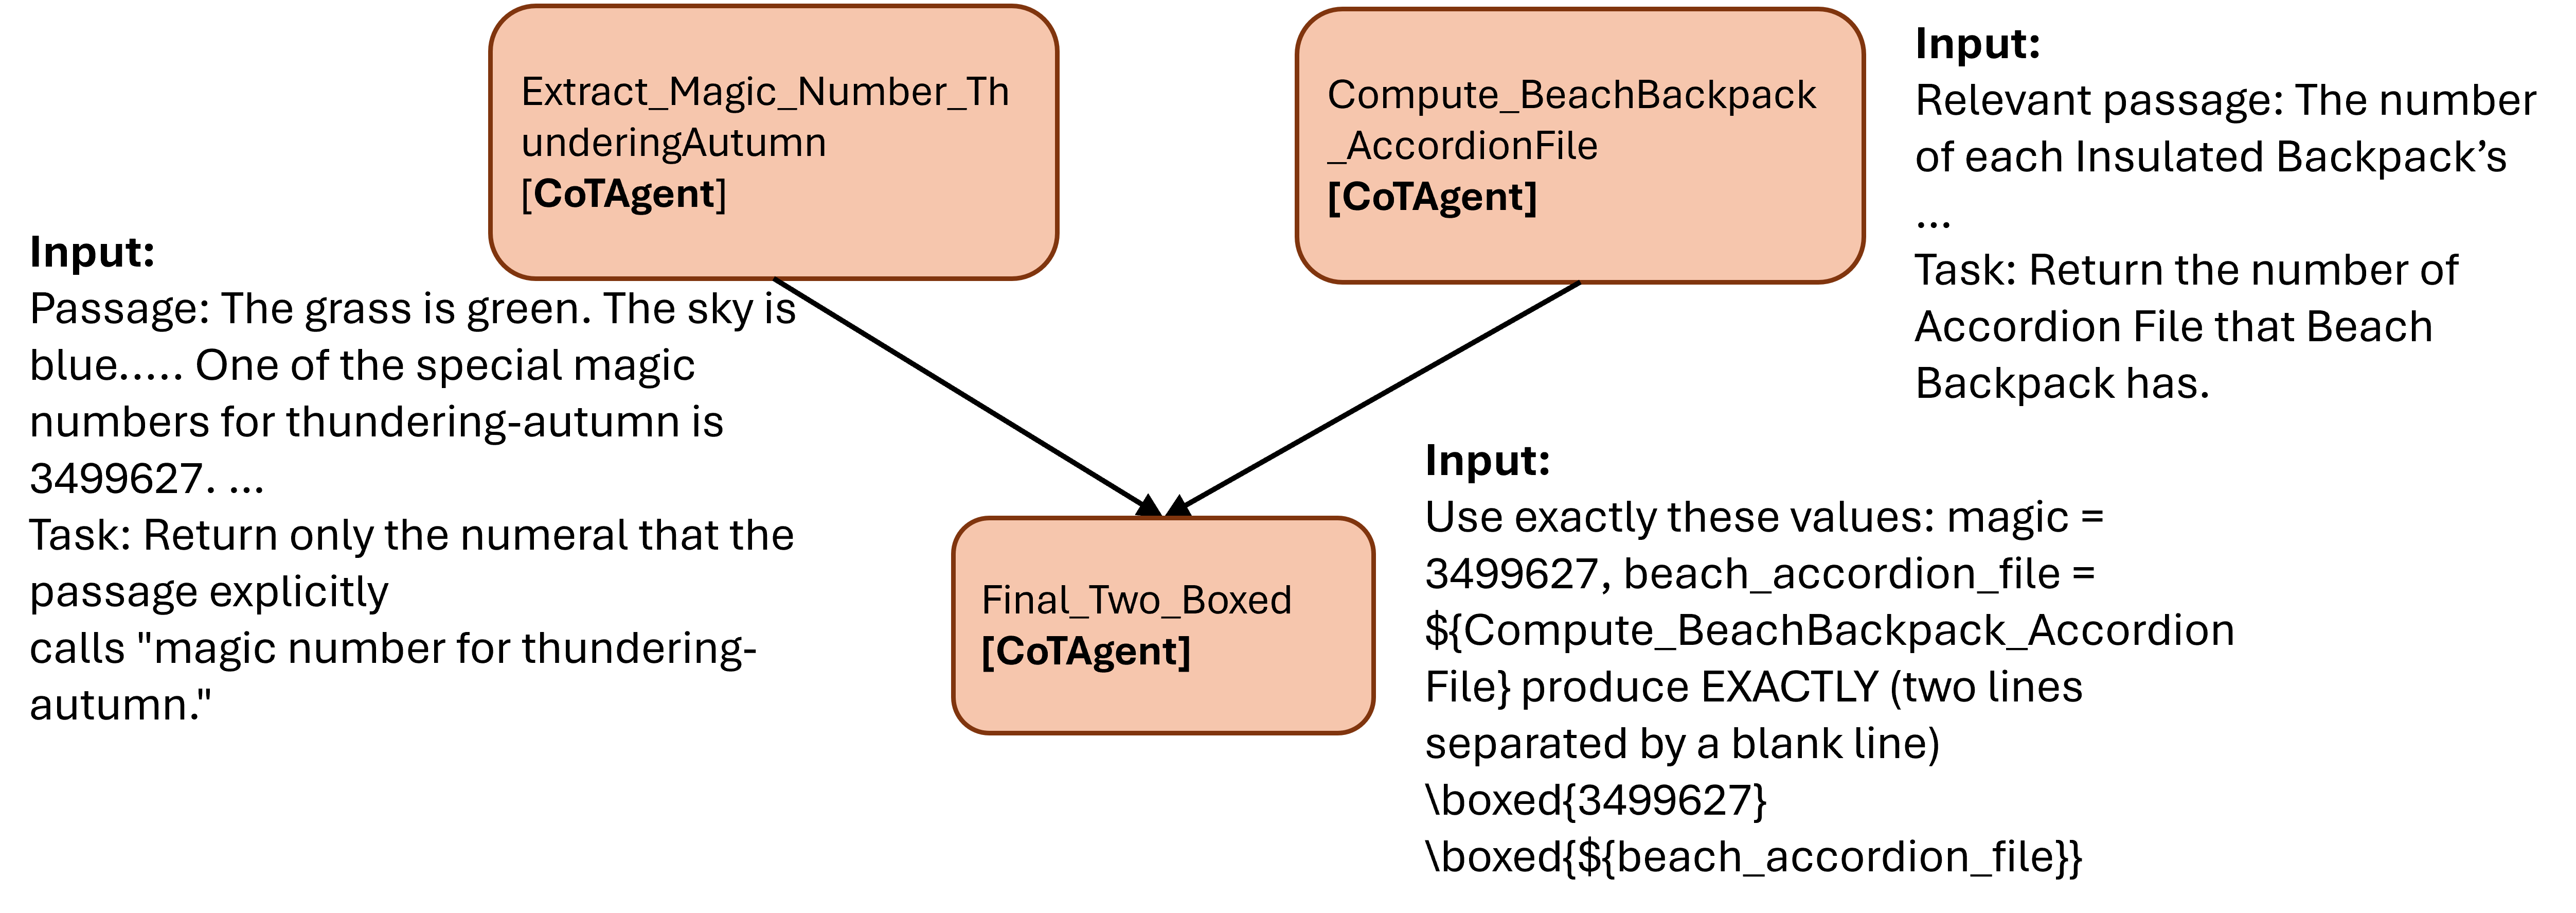
\includegraphics[height=4.1cm]{figs/sas_vs_mas.png}}
\\
\midrule
\textbf{Execution Output}
&
\boxed{7381734}

\boxed{42}
&
\boxed{3499627}  

\boxed{19}
\\
\midrule
\textbf{Ground Truth Answer}
& \multicolumn{2}{c}{
\boxed{3499627} \boxed{19}
} \\
\bottomrule
\end{tabularx}
\caption{Comparison of Single-agent System (SAS) and Multi-agent System (MAS) on the same problem instance. 
% \zixuan{where is this sample from}
}
% from https://vincent950129.github.io/mas-design/mas_r1/qwen2.5_7b_oss_120b_low_conflict2.html and call GPT-OSS at real time
\label{tab:sas_mas_example}
\end{table*}


% \zixuan{working}
\subsection{Robustness and Adversarial-aware Training.} Importantly, performance on the \robustness axis in \cref{fig:mas_combined_comparison} incorporate {combined training data that include} adversarial examples. In practice, however, such examples is often unavailable or omitted. To study this effect, \cref{fig:robustness_combine} compares models
trained {on combined data} with and without adversarial examples. We observe that when adversarial data is excluded, performance on the \robustness axis remains poor (nearly
zero and comparable to SAS performance in \cref{fig:robustness}). This result
indicates that while combined training generalizes well across most axes, it
fails to generalize to robustness. Explicit inclusion of adversarial data is therefore necessary to improve robustness performance.


\textbf{Remark.} Separate training and combined training require different numbers of training
steps, as the combined dataset is naturally larger. The goal of our experiments
is not to fully converge in the RL training, but rather to
examine how different factors affect the performance of MAS. In our experiments,
we allocate twice as many training steps for combined training compared to
separate training. We expect that further performance gains are possible for
combined training with additional training steps.


%%%%%%%%%%%%%%%%%%%%%%%%%%%%%%

\subsection{Statistics of Agents for All Axes}

{\cref{fig:axes_detail} reports detailed statistics about the total number of sub-agents generated for different evaluation axes (\depth, \horizon,\ breadth, \myparallel and \robustness).} These results show that the orchestrator can largely learn to mirror the underlying task structure in its orchestration design. However, this structural alignment does not necessarily translate into performance gains over SAS, {as discussed earlier}.

% \cref{fig:axes_detail} shows detailed statistics of the total number of sub-agents generated under different evaluation axes (\depth, \horizon, \breadth, \myparallel, and \robustness), using \qwen as the orchestrator and \ossonetwenty as the sub-agent.

\begin{figure*}[h!]
\centering
% \vspace{-2\baselineskip}
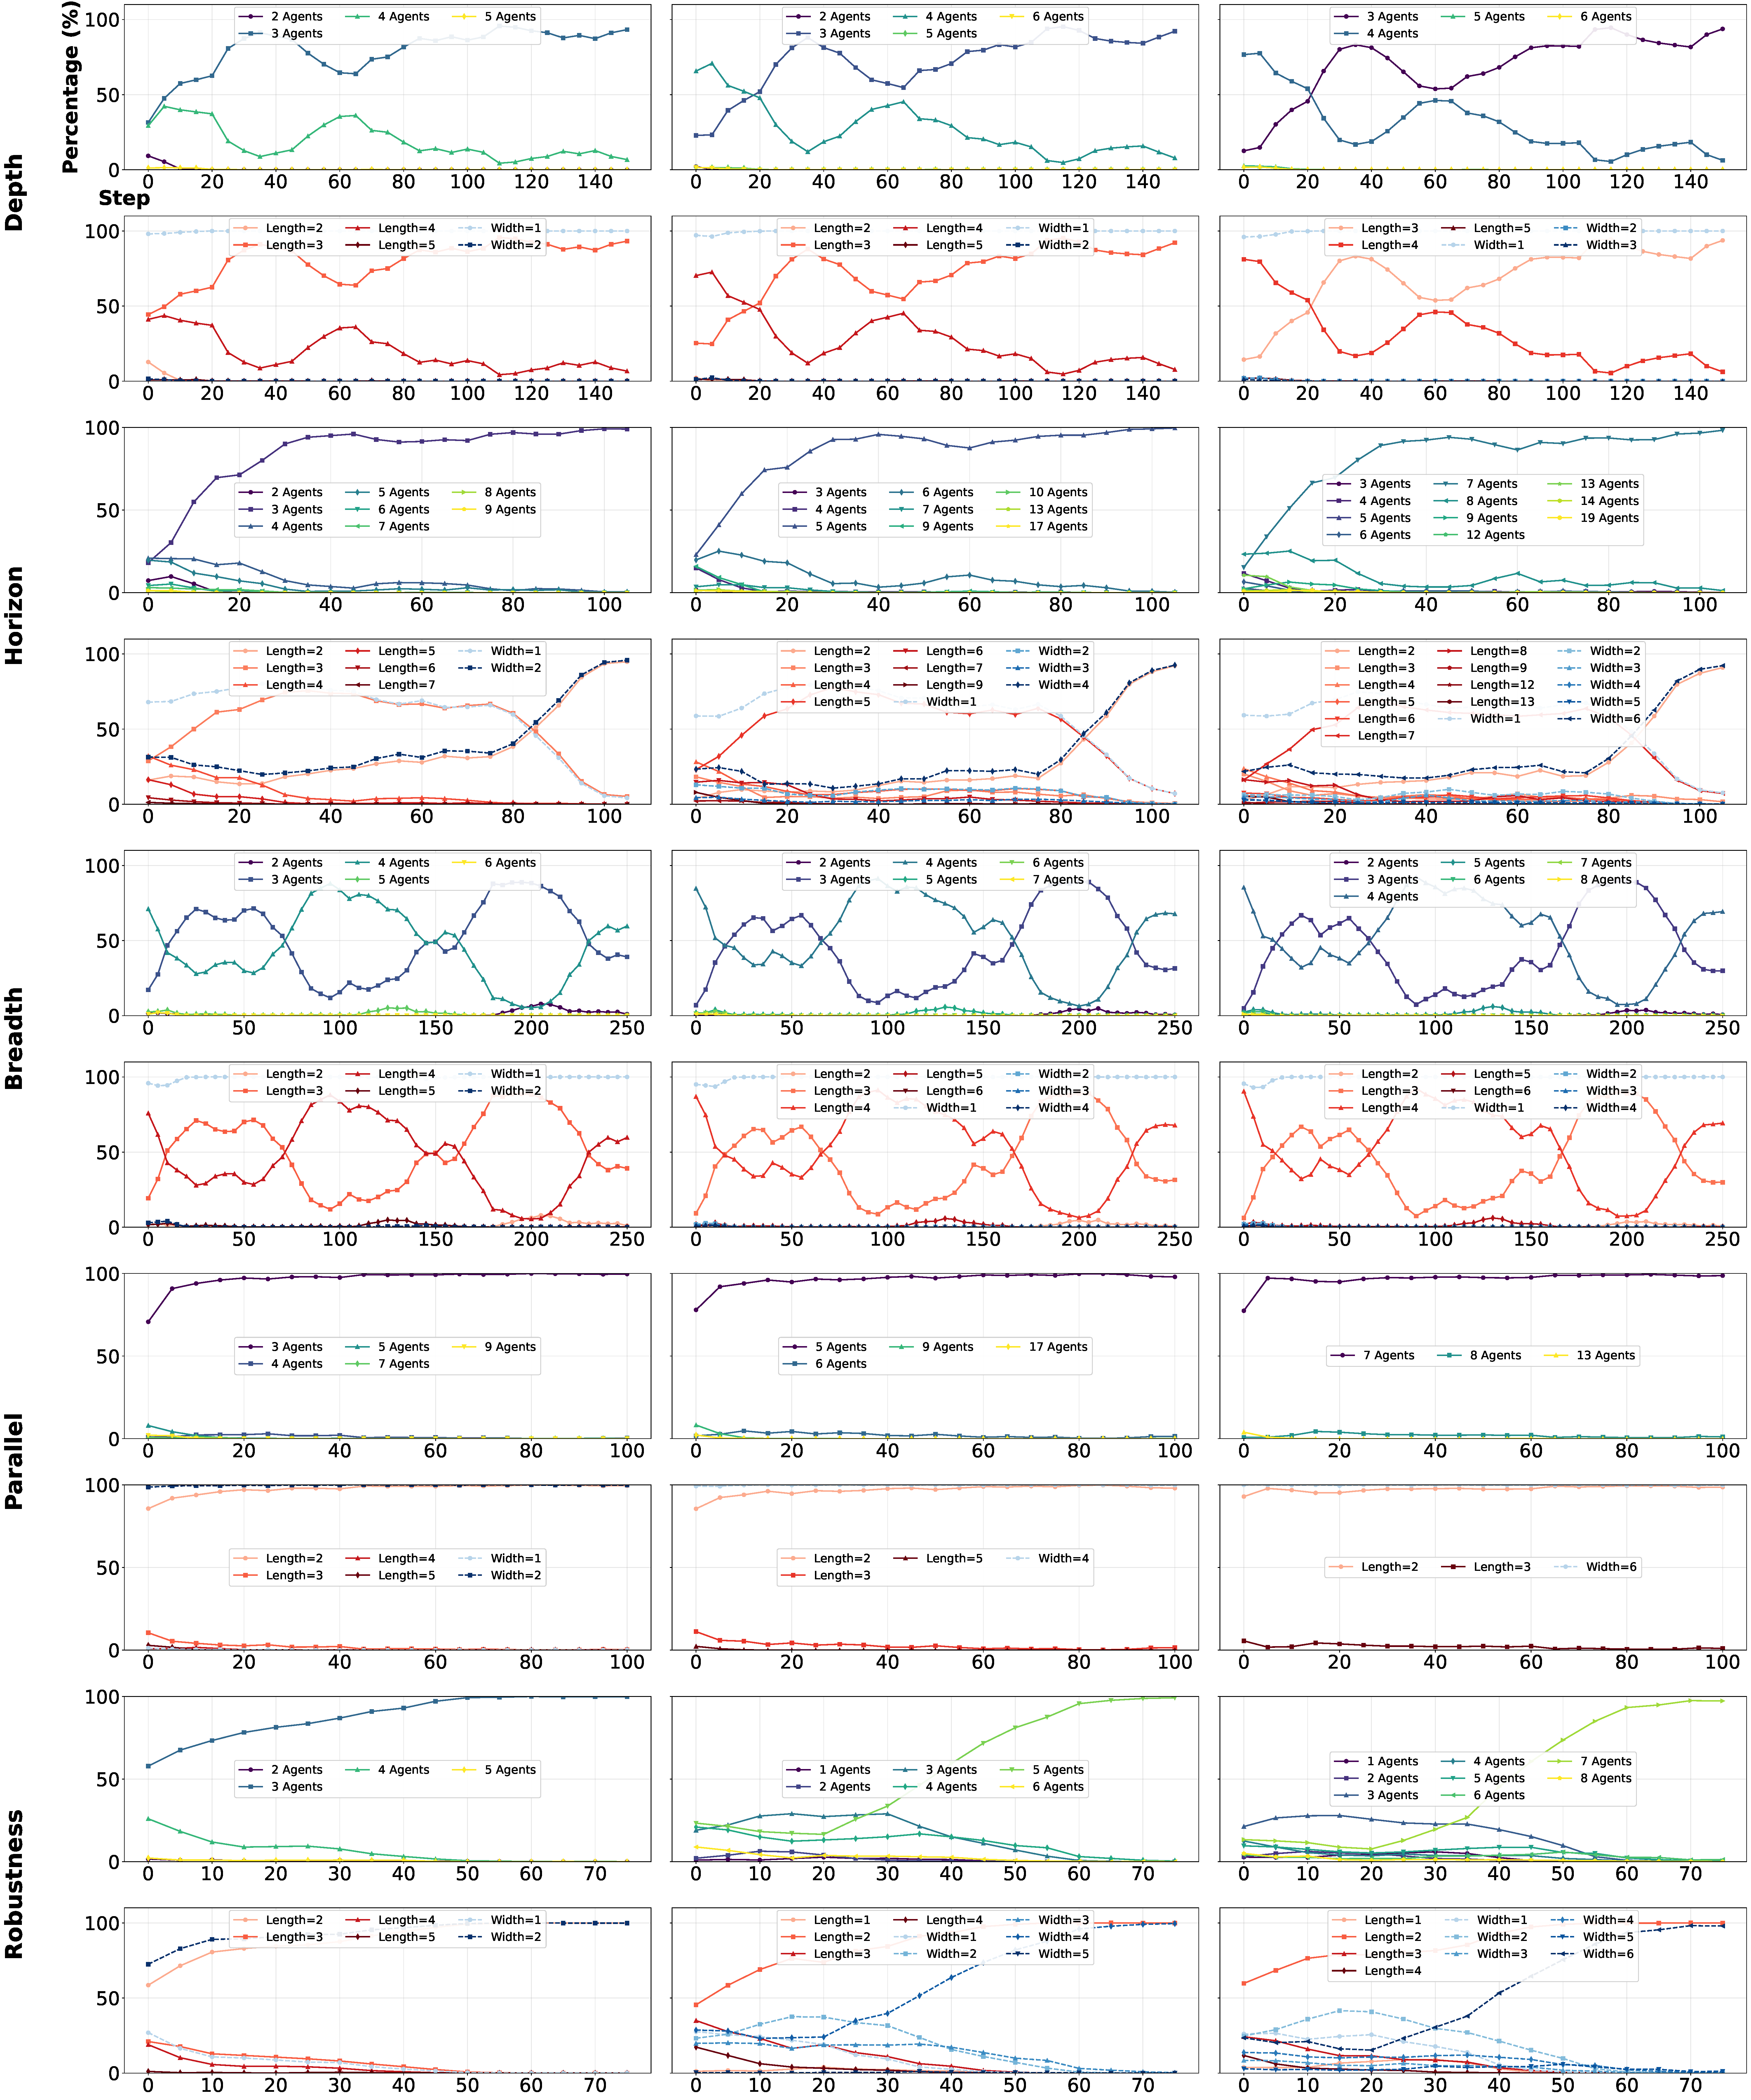
\includegraphics[width=\columnwidth]{figs/7b_120b_low_combine.pdf}
\vspace{-\baselineskip}
\captionof{figure}{\small Statistics of agents for different axes (the correspnding values are 2, 4, 6 from left to right).}
\label{fig:axes_detail}
\end{figure*}

% As discussed in \cref{sec:subtask_structure}, overall, these results show that the orchestrator can largely learn to mirror the underlying task structure in its orchestration design. 

Below, we provide several detailed observations.

\subsubsection{Given Axes, Observations Across Values.}

We first examine observations within a given axis. As task complexity increases (i.e., as the axis value becomes larger), \textbf{more sub-agents are generated}. This behavior is expected and indicates that the orchestrator effectively adapts to increasing task complexity.

We further observe that, within the same axis, the overall orchestration pattern remains similar across different values, despite the increase in the number of sub-agents. This suggests that the \textbf{orchestrator is stable} with respect to its learned structural strategy and scales the number of sub-agents without changing the underlying orchestration structure as task complexity increases.

% whereas \myparallel and \horizon exhibit more diverse multi-agent structures.

% We observed that \depth and \breadth tends converg to a general sequential (i.e., \text{Parse → Solve → Verify → Final Answer}), while \myparallel parallel MAS and Horizon is relatively more diverse.


% MAS Pattern: Depth and Breadth converged to a general sequential (Parse → Solve → Verify → Final Answer). Parallel converges to parallel MAS and Horizon is relatively more diverse.

\subsubsection{Given Value, Observations Across Axes.}

We observe that \depth and \breadth tend to converge to a general sequential pattern. Specifically, the length typically ranges from 1 to 5, while the width remains much smaller, usually up to 2. A closer inspection of the generated examples shows that the resulting MAS commonly follows a structure of \text{Parse} $\rightarrow$ \text{Solve} $\rightarrow$ \text{Verify} $\rightarrow$ \text{Final Answer}. This indicates that, for tasks with sequential dependency chains or fan-in structure, a linear decomposition with explicit intermediate reasoning is sufficient and stable under the given setting.

In contrast, \myparallel tends to converge to parallel MAS structures, where the width is typically aligned with the specified \myparallel value. This behavior closely mirrors the underlying task structure and suggests that the orchestrator can effectively learn and exploit independent sub-task structures under the current training method.

For \horizon, the observed structural diversity reflects uncertainty about when intermediate results should be made explicit. Some tasks benefit from early synthesis of partial answers, whereas others require delayed aggregation after several reasoning steps. The orchestrator adapts by varying both the number and the ordering of sub-agents across horizon settings, suggesting that \ourframework learns temporal control strategies from task-level feedback rather than relying on a fixed reasoning depth.

For \robustness, we observe a tendency toward parallel MAS structures. This orchestration strategy allows different sub-agents to address different sub-tasks and helps isolate and mitigate adversarial or incorrect information, either within individual sub-agents or through additional verification or moderation components.


% We observe that \depth and \breadth tend to converge to a general sequential pattern (i.e., length ranges from 1 to 5 while the width is much smaller, usualy up to 2. A further look at example can be foudn that the geenrataer MAS is typrcially \text{Parse} $\rightarrow$ \text{Solve} $\rightarrow$ \text{Verify} $\rightarrow$ \text{Final Answer}), indicating that for tasks with long dependency chains or large fan-in, a linear decomposition with explicit intermediate reasoning is both sufficient and stable for the given setting. \myparallel tebnd to converge to parallel MAS (wideht typically the same as the \parallel value), clealry mirror the task structure, indicating that it is suffiicent to learn the indendepcnt t structuire ia current method. In contrast, For \horizon, the observed diversity reflects uncertainty about when intermediate results should be made explicit. Some tasks benefit from early synthesis of partial answers, while others require delayed aggregation after several reasoning steps. The orchestrator adapts by varying both the number and ordering of sub-agents across horizon settings, suggesting that \ourframework learns temporal control strategies based on task feedback rather than relying on a fixed reasoning depth. For \robstuness, we observat that it tend to concerge to parallel MAS, which is a smart orchesttation that can enable diffetnet sub-agent address different sub-task and effeictively handle the adversatial information within individual sub-agent or an additional moderatotrr.

% MAS Pattern: conflict convereges to parallel MAS


% \zixuan{maybe we can use table with figures}

% \begin{table*}[h]
% \centering
% \small
% \setlength{\tabcolsep}{6pt}
% \renewcommand{\arraystretch}{1.05}
% \begin{tabular}{c m{0.27\textwidth} m{0.27\textwidth} m{0.27\textwidth}}
% \toprule
% \textbf{Axis} & \textbf{Value = 2} & \textbf{Value = 4} & \textbf{Value = 6} \\
% \midrule

% Depth &
% \includegraphics[width=\linewidth]{figs/7b_120b_low_individual_depth2.pdf} &
% \includegraphics[width=\linewidth]{figs/7b_120b_low_individual_depth4.pdf} &
% \includegraphics[width=\linewidth]{figs/7b_120b_low_individual_depth6.pdf} \\[-2pt]

% Horizon &
% \includegraphics[width=\linewidth]{figs/7b_120b_low_individual_horizon2.pdf} &
% \includegraphics[width=\linewidth]{figs/7b_120b_low_individual_horizon4.pdf} &
% \includegraphics[width=\linewidth]{figs/7b_120b_low_individual_horizon6.pdf} \\[-2pt]

% Breadth &
% \includegraphics[width=\linewidth]{figs/7b_120b_low_individual_breadth2.pdf} &
% \includegraphics[width=\linewidth]{figs/7b_120b_low_individual_breadth4.pdf} &
% \includegraphics[width=\linewidth]{figs/7b_120b_low_individual_breadth6.pdf} \\[-2pt]

% Parallel &
% \includegraphics[width=\linewidth]{figs/7b_120b_low_individual_parallel2.pdf} &
% \includegraphics[width=\linewidth]{figs/7b_120b_low_individual_parallel4.pdf} &
% \includegraphics[width=\linewidth]{figs/7b_120b_low_individual_parallel6.pdf} \\[-2pt]

% Robustness &
% \includegraphics[width=\linewidth]{figs/7b_120b_low_individual_conflict2.pdf} &
% \includegraphics[width=\linewidth]{figs/7b_120b_low_individual_conflict4.pdf} &
% \includegraphics[width=\linewidth]{figs/7b_120b_low_individual_conflict6.pdf} \\

% \bottomrule
% \end{tabular}
% \end{table*}
% \zixuan{may need to draw a big figure instead, too small}


% \zixuan{TODO: put results for combination training here}


\subsection{Separate vs. combined training.} 

% \subsection{Separate vs. Combined training.} 
In \cref{fig:sub_task_sub_agent}, we train the orchestrators using training
data from different axes. Now, we examine: \textit{can data from different axes be combined for
training, and can the resulting orchestrator generalize when tested on
individual axes?} \cref{fig:mas_combined_comparison} reports results obtained by training on
combined data from all five axes. We observe that the
performance across different axes is highly similar, indicating that the
 the orchestrator can effectively generalize when
trained on combined data. 



% In \cref{fig:mas_combined_comparison}, we demonstrate results obtained by training on combined data from all five axes. See \cref{sec:subtask_structure} for detailed descriptions and observation.

% In \cref{fig:sub_task_sub_agent}, we train the orchestrators using training
% data from different axes. Now, we examine: \textbf{can data from different axes be combined for
% training, and can the resulting orchestrator generalize when tested on
% individual axes?} \cref{fig:mas_combined_comparison} reports results obtained by training on
% combined data from all four axes (excluding \robustness). We observe that the
% performance across different axes is highly similar, indicating that the
%  the orchestrator can effectively generalize when
% trained on combined data from multiple axes. 

% \shafiq{If the robustness results reported before and in Fig 4 (without combined) with training on robustness, we need to reorganize this section. Let's talk about this.} \zixuan{TODO: first talk about combine has the same observation as individual, and then discuss that removing robustness data will cause significant degrade on robustness (details move to Appendix \cref{ap:discuss_combine_training} as the observation is similar as individual)}

\begin{center}
\vspace{-0.5\baselineskip}
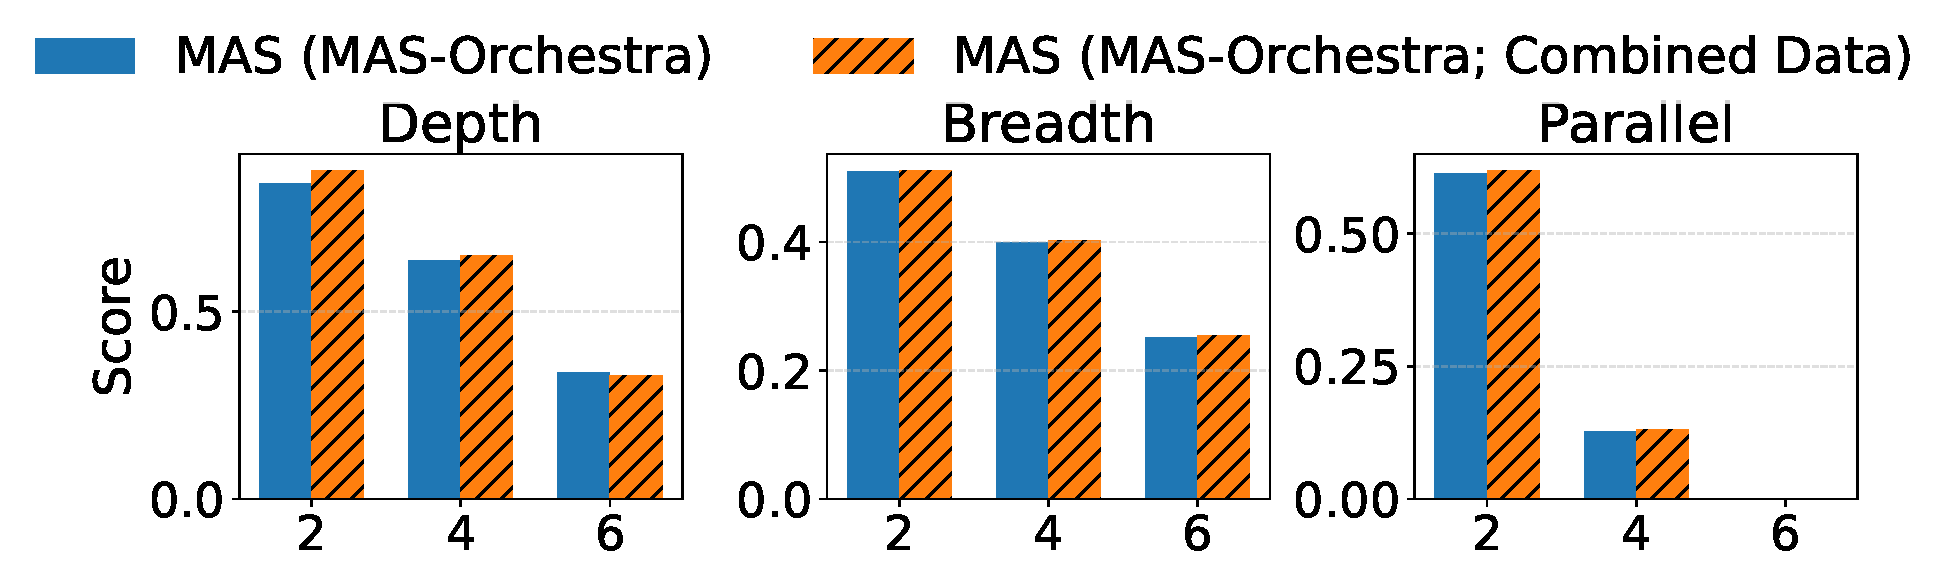
\includegraphics[width=0.6\columnwidth]{figs/mas_combined_comparison.pdf}
\vspace{-10pt}
\captionof{figure}{\small \avgat{8} comparing separate and combined training. 
% \shafiq{why there is no horizon?}\zixuan{the combine experiemtns is not as complete as individual, will move to Appendix}\zixuan{still missing at the moment}
}
% \zixuan{TODO: add robustness as well: canot generalize to robustness}
\label{fig:mas_combined_comparison}
\end{center}




\textbf{\robustness.} 
% A straightforward way to address the above issue is to incorporate robustness
% training data during training. 
\cref{fig:robustness_combine} compares models
trained on the combined data, with and without adversarial samples. We observe that incorporating adversarial training data leads to a substantial improvement over training without such
data. This result indicates that explicitly including adversarial examples in the combined training data is
necessary for improving robustness performance.


\begin{center}
% \vspace{-0.5\baselineskip}
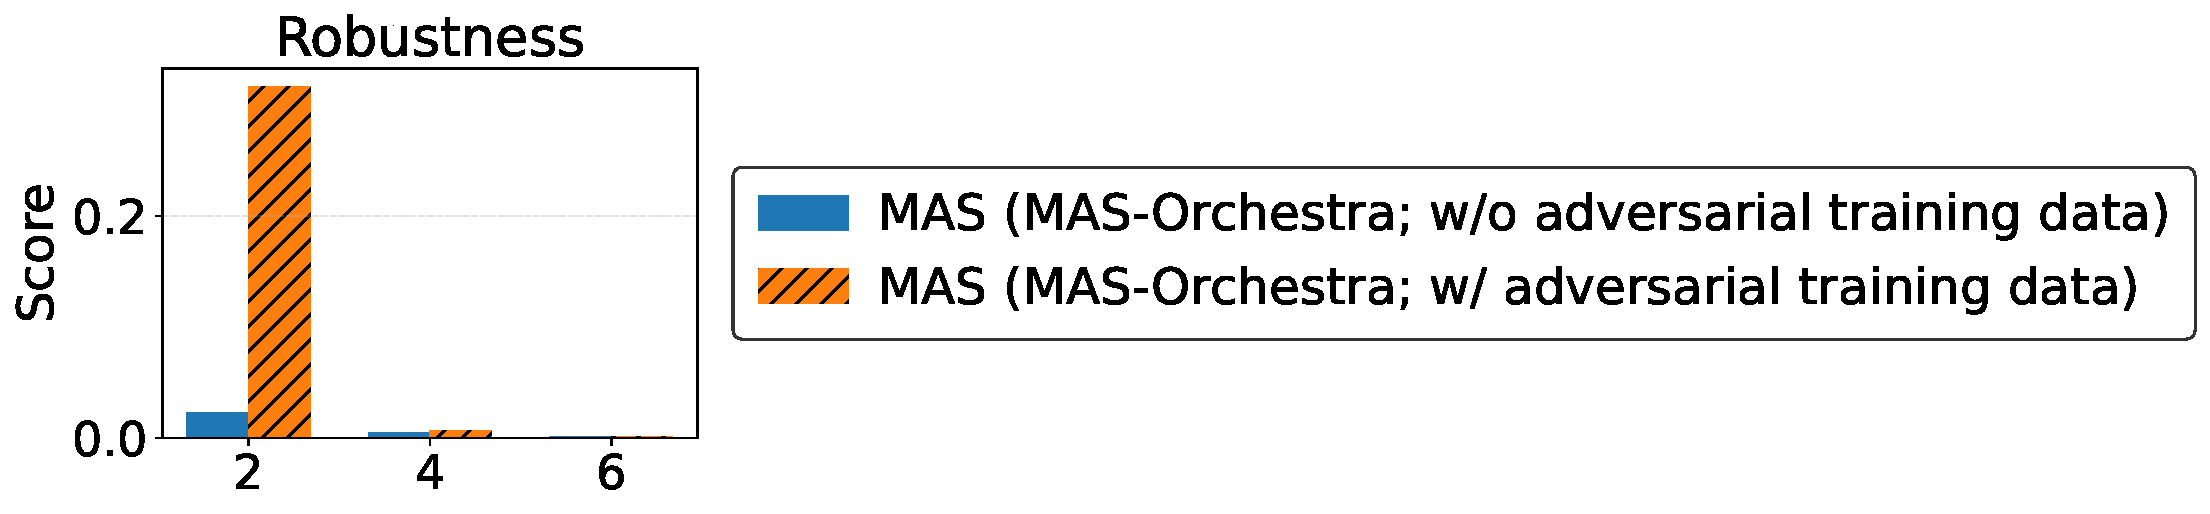
\includegraphics[width=0.6\columnwidth]{figs/oss120b_robustness_combine.pdf}
\vspace{-0.5\baselineskip}
\captionof{figure}{\small \avgat{8} of \robustness combined training w/ and w/o adversarial-aware training}
\label{fig:robustness_combine}
\end{center}

% \shafiq{If we need space, this can go to Appendix with a brief summary in the main body. Let's talk}

% \subsection{Does RLM orchestrator size affect MAS performance?}
\subsection{How Does RLM Orchestrator Size Affect MAS Performance?} 

Since \qwen is a 7b model while the RLM used above has 20b  parameters, one may
wonder whether model size plays a role in the observed performance gap. To
investigate this, we compare a 7b RLM DeepSeek-R1-Distill-Qwen-7B (\deepseekqwen) \cite{deepseekai2025deepseekr1incentivizingreasoningcapability} with \qwen under
combined training, using a similar number of training steps. As shown in
\cref{fig:deepseek}, even when controlling for model size, the RLM consistently underperforms the LLM across different axes. This result suggests that the
current RLM is not well suited to serve as an orchestrator. 

% \shafiq{If we need space, this can go to Appendix with a brief summary in the main body}

\cref{fig:deepseek} compares performance when using the same-size instruction-tuned LLM versus RLM. A detailed description is provided in \cref{sec:reasoning_meta_agent}.

\begin{center}
\vspace{-0.5\baselineskip}
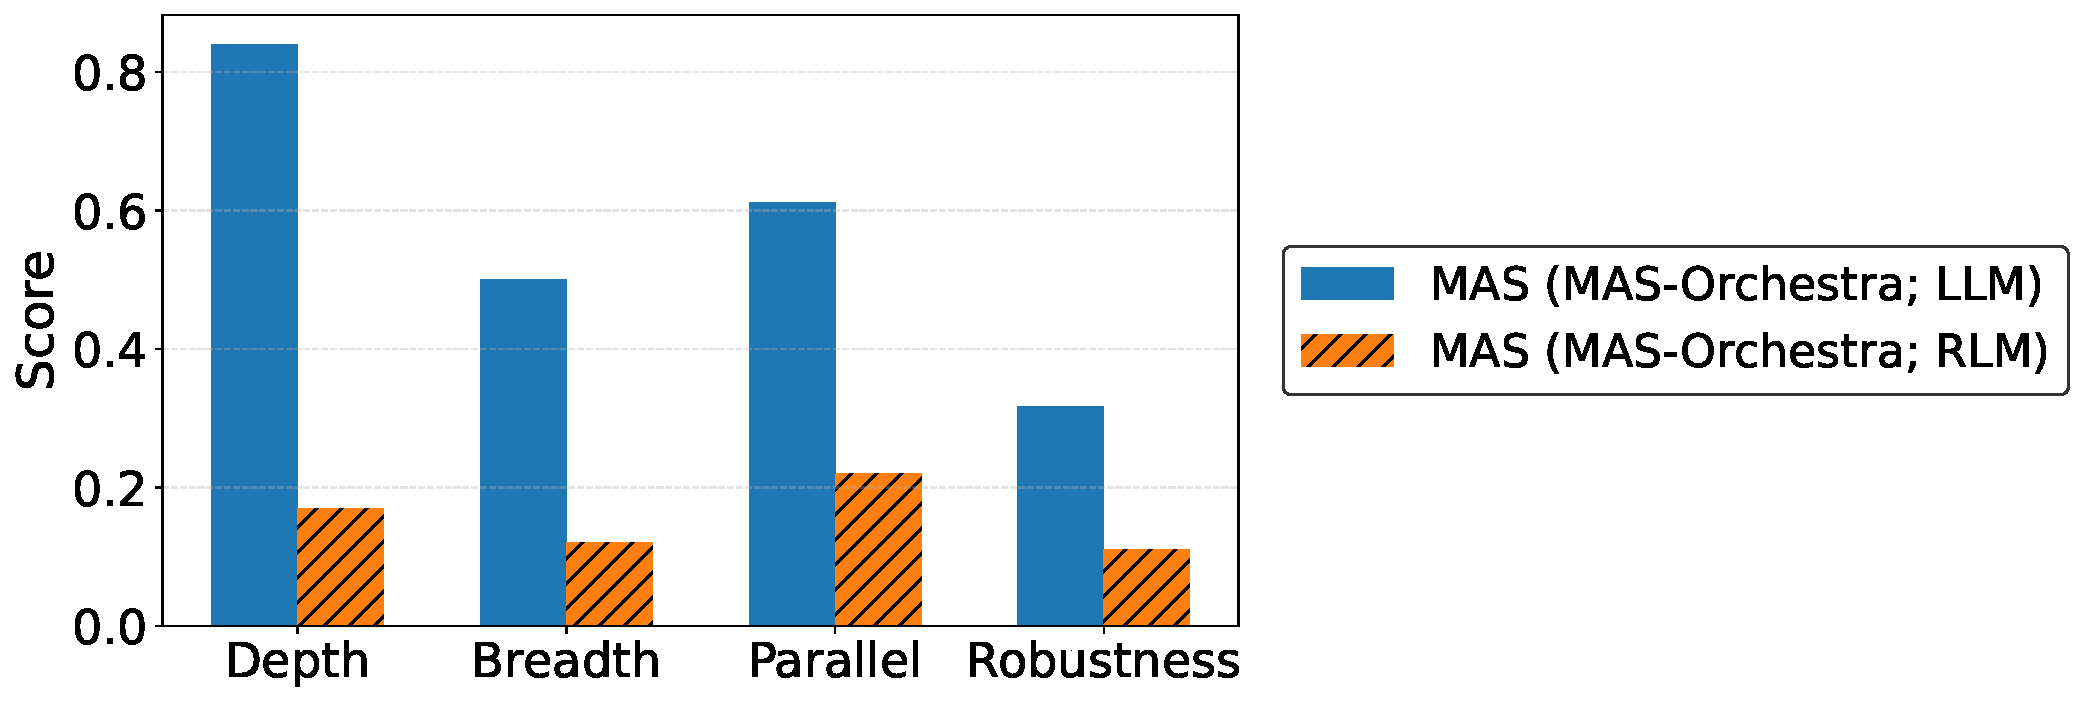
\includegraphics[width=0.6\columnwidth]{figs/deepseek.pdf}
% \vspace{-\baselineskip}
\captionof{figure}{\small \avgat{8} comparing LLM (\qwen) and RLM (\deepseekqwen) \textbf{with the same size} as orchestrator.}
\label{fig:deepseek}
\end{center}

\subsection{Complexity Generalization}
\label{ap:complexity_generalization}

% To facilitate the investigation of  \textit{complexity generalization}, we train the orchestrator on instances with smaller axis values and evaluate on both the training values and higher, held-out axis values in \ourbenchmark. Additional discussion is provided in \cref{ap:complexity_generalization}, and further
 
To facilitate the investigation of  \textit{complexity generalization}, we train the orchestrator on instances with smaller axis values and evaluate on both the training values and higher, held-out axis values in \ourbenchmark. {Specifically, the model is trained on \depth values from 2 to 8 and evaluated up to 12. For \breadth and \myparallel, training covers values from 2 to 4, with evaluation extending to 8. For \horizon and \robustness, training values range from 2 to 6, and evaluation values range up to 8.} 

As the tasks become more complex, performance decreases. Importantly, out-of-distribution complexity follows the same trend as in-distribution complexity.
This suggests that \ourframework induces controlled increases in
task complexity and exhibits consistent generalization behavior as the task
complexity grows. 
% \zixuan{can move to appendix}



\subsection{LLM vs. RLM as Orchestrator}
\label{ap:rlm_orchestrator}


\textbf{Statistics of Agents.} \cref{fig:7b_120b_vs_20b_120b_depth4} shows agent statistics in the
MAS proposed by MAS-Orchestra. See \cref{sec:reasoning_meta_agent} for detailed descriptions and observations.

\begin{center}
\vspace{-0.5\baselineskip}
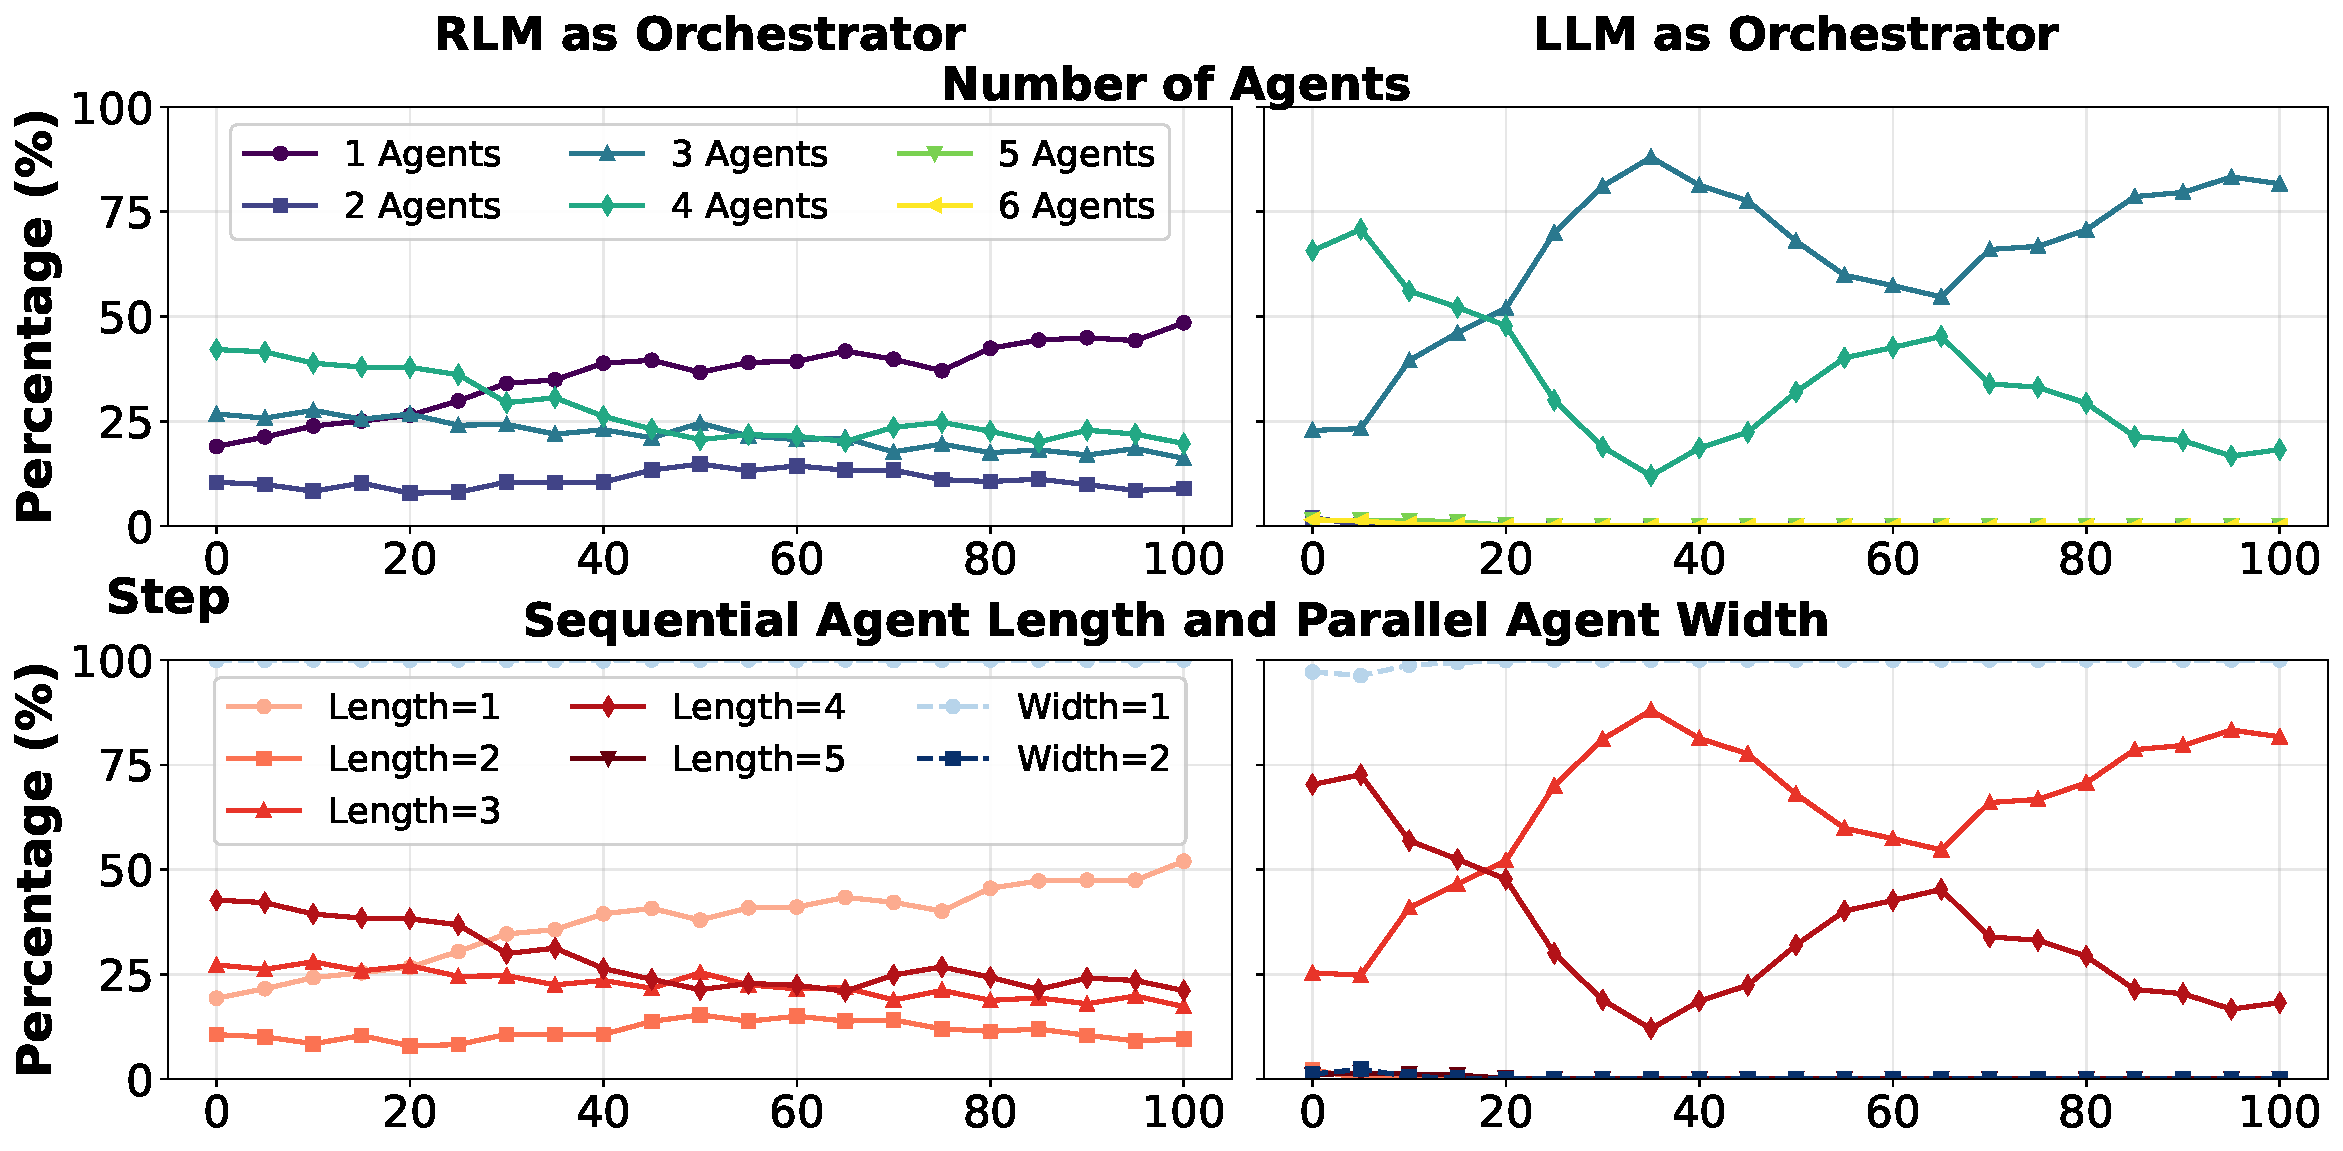
\includegraphics[width=0.8\columnwidth]{figs/7b_120b_vs_20b_120b_depth4.pdf}
% \vspace{-\baselineskip}
\captionof{figure}{\small Statistics of agents in the generated MAS over the training steps (use \depth equals 4 as an example). {The \textit{number of agents} measures the total number of sub-agents, the \textit{sequential agent length} measures  the length of dependency chain  and \textit{parallel agent width} measures the in degree of sub-agent.}}
\label{fig:7b_120b_vs_20b_120b_depth4}
\end{center}




\textbf{Example.}
In \cref{tab:rlm_example}, we demonstrate a sample from the \depth axis (\depth equals to 4) using \qwen as the orchestrator and \ossonetwenty as the sub-agent. See \cref{sec:reasoning_meta_agent} for detailed descriptions and observations.


% \zixuan{if it is not compare, we may not use table, or add compare,s horten tables}
% \zixuan{consider long table}
\begin{table*}[h!]
\centering
\small
% \addtolength{\tabcolsep}{-0.4em}
\begin{tabularx}{\textwidth}{l X X}
\toprule
\textbf{Orchestrator} & \textbf{\osstwenty} & \textbf{\qwen}\\
\midrule
\textbf{Problem} & \multicolumn{2}{p{0.76\linewidth}}{
 The number of each Golden Gate Park in San Francisco's Anteater equals 21. The number of each Bois de Boulogne in Paris's Kangaroo equals each Chapultepec Park in Mexico City's Wolf. The number of each Bois de Boulogne in Paris's Wolf equals 6. .... How many Moose does Chapultepec Park in Mexico City have?}\\
\midrule
\textbf{Thinking} &
analysisWe need to design agents. Problem: find number of Moose in Chapultepec Park in Mexico City. Let's parse quickly.

Variables: Let's denote:

GGP_SF_Anteater = 21 (given)
GGP_SF_Wolf = 12
GGP_SF_Moose = ?
GGP_SF_Kangaroo = ?
GGP_SF_Moose equals each Chapultepec Park in Mexico City's Wolf. So GGP_SF_Moose = CP_MX_Wolf.

...

No other constraints involve CP_MX_Creatures. So no issue.

Thus answer 42.

We can create single agent? Single agent can solve. But we may want multi-agent to show reasoning. However constraints allow single agent. But we can do multi-agent for demonstration.

Simpler: one CoTAgent with empty input to solve directly. That is simplest. But we must ensure final answer. Provide final agent with empty input. That yields final answer.

But we might want to show intermediate steps? Not necessary.

Given we can do single agent. Let's do single agent.

...

Let's produce.

assistantfinal<thinking>
  The problem is a straightforward system of linear equations with a single unknown of interest: the number of Moose in Chapultepec Park, Mexico City.  
  All other variables are either given directly or can be expressed in terms of the known constants.  
  A single CoTAgent can parse the statements, instantiate the variables, perform the necessary substitutions, and produce the final numeric answer.  
  Since no intermediate agents are needed, the graph consists of just this one sink agent, which also serves as the start node. 
  & 
  <thinking>
  This problem involves setting up and solving a system of equations. Using a single agent would be insufficient as it would mix the steps of parsing the problem and solving it, increasing the risk of errors. We need to parse the problem into equations first, then solve the system of equations, and finally verify the solution. This separation ensures accuracy and allows for independent verification of each step.
  The final answer will be provided by the Final_Answer agent.
\\
\midrule
\textbf{Execution Output} &
21
&
19
\\
\midrule
\textbf{Ground Truth Answer} & \multicolumn{2}{c}{
19}
\\
\bottomrule
\end{tabularx}
\caption{Comparison of instruction-tuned LLM (\qwen) and RLM (\osstwenty) on the same problem instance.
% \osstwenty as orchestrator run on one problem instance, including the model output and the ground truth answer.
}
% from https://vincent950129.github.io/mas-design/mas_r1/qwen2.5_20b_oss_120b_low_depth4.html
\label{tab:rlm_example}
\end{table*}



\subsection{\robustness under high reasoning effort when context lengths are longer} 


\begin{center}
\vspace{-0.5\baselineskip}
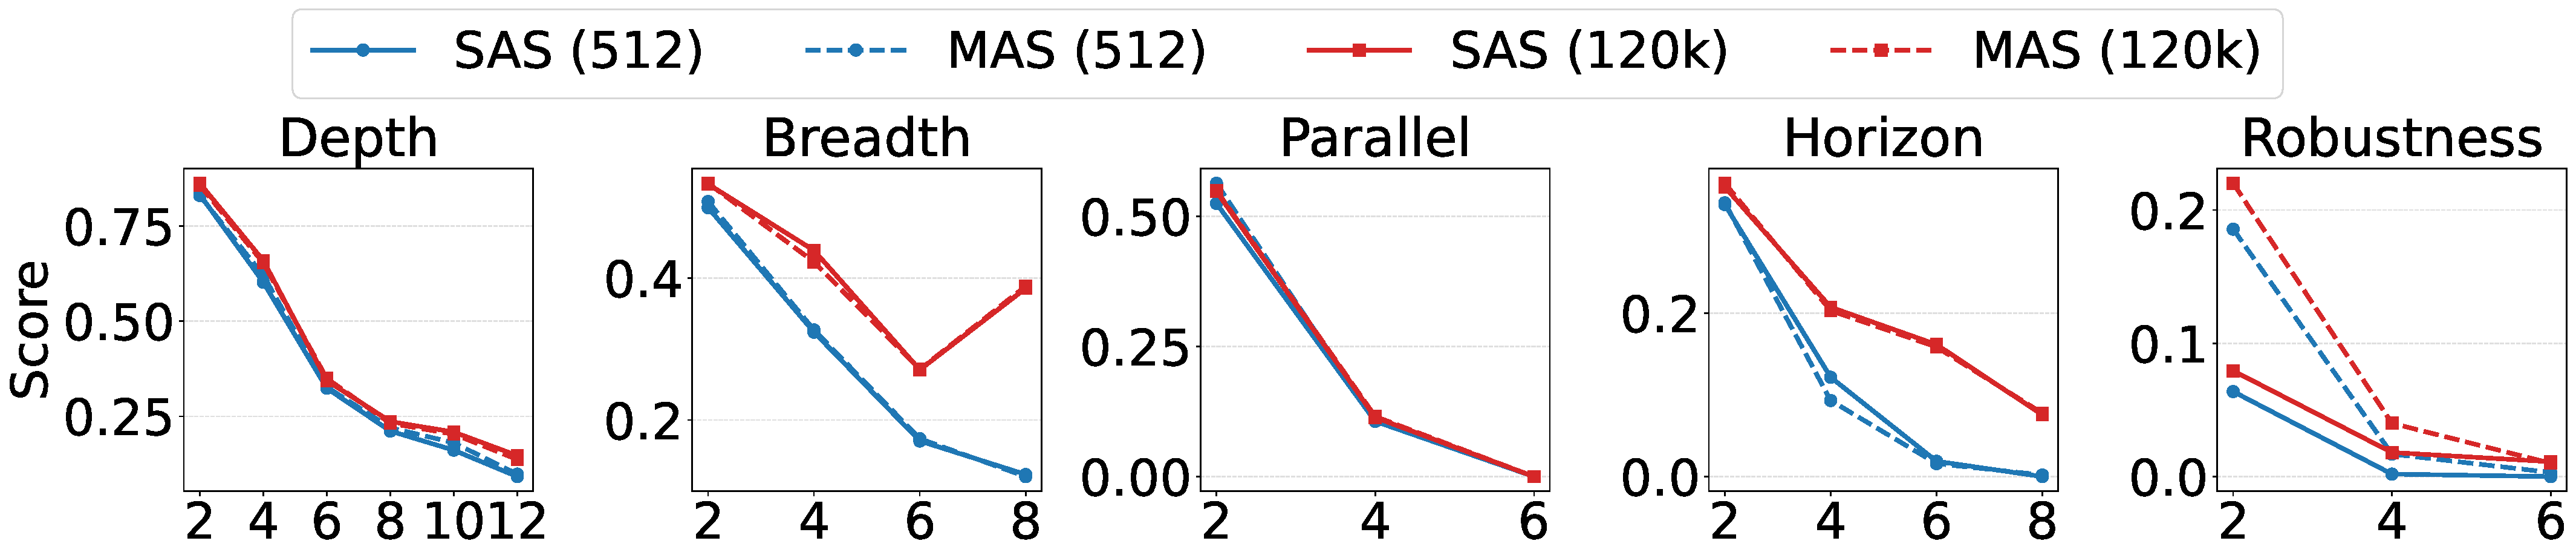
\includegraphics[width=\columnwidth]{figs/max_length.pdf}
\vspace{-\baselineskip}
\captionof{figure}{\small \avgat{8} comparing different maximum context length with \qwen as orchestrator and \ossonetwenty as sub-agent.}
\label{fig:max_length}
\end{center}
